\chapter{Performance Challenges with Java Big Data Analytics} \label{sec:perfchallenges}
Big data applications pose numerous challenges from data storage to communication, and to processing. This section identifies the performance challenges with Java big data analytic applications and presents how some of these were solved in SPIDAL Java using clever optimization techniques. While some of the optimizations are specific to SPIDAL Java, they can be used as general guidelines in developing other Java based big data applications.


\section{Intra-node Communication}
With increasing core counts per node comes the challenge of efficiently exploiting all cores with minimum overhead. Three approaches exist in 
\section{Cost of Threads}
\section{\acl{NUMA} and Cache Effects}

\section{\acl{GC} Cost}

\section{Data Serialization and Deserialization}
default serialization is verbose - show with some example
then about arrays - better but 1D is the best

\section{Data Read Write}
can mention about slowness in streaming I/O compared to mmap bulk loading







\section{Intra-node Communication}
Intra-node communication on large multicore nodes causes a significant performance loss. Shared memory approaches have been studied as successful alternatives in Message Passing Interface (MPI) oriented researches \cite{lechai},\cite{Wickramasinghe:2014:HMC:2612262.2612267}, and \cite{Li:2013:NSC:2493123.2462903}, however, none are available for Java. Also, popular big data frameworks too uses TCP for intra-node communications, which is prohibitively expensive for applications in SPIDAL Java.

SPIDAL Java uses OpenMPI for inter-node communication, but its shared memory support is very limited and does not include collectives such as variants of \texttt{allgather}, which is used in multidimensional scaling applications.

\begin{figure}[!h]
\centering
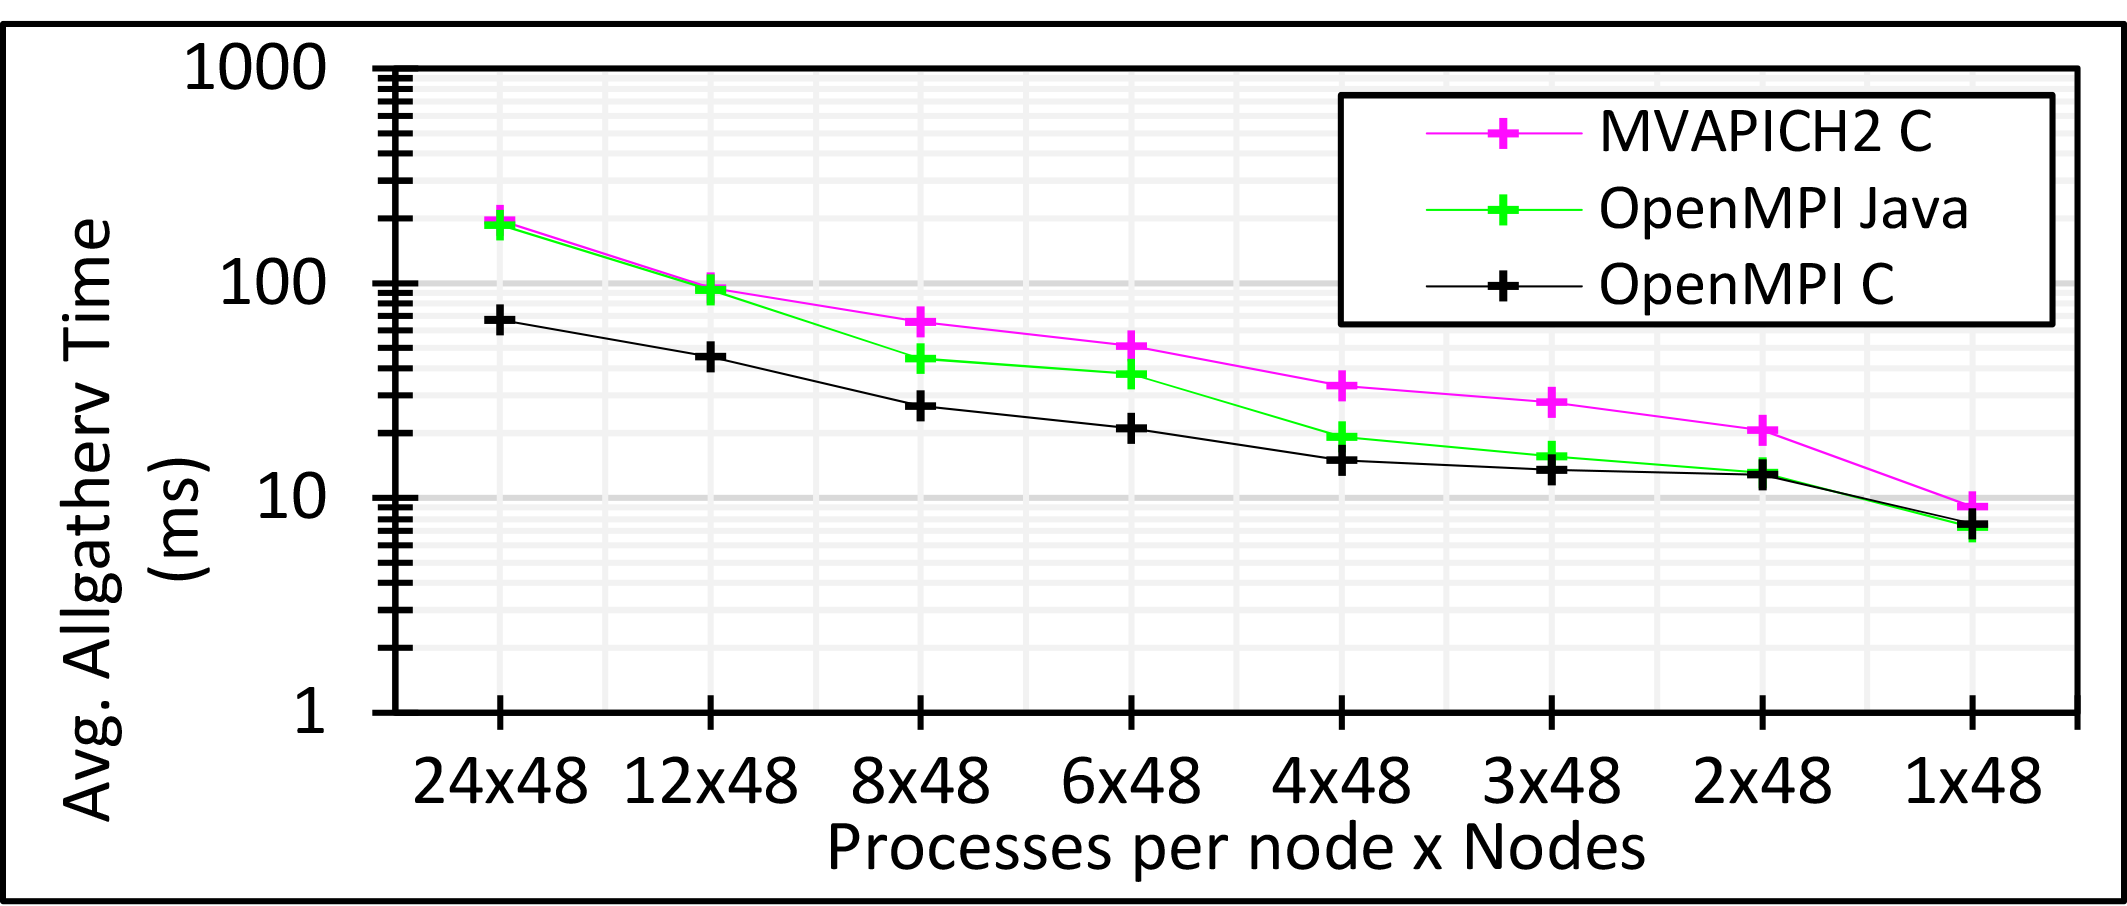
\includegraphics[width=0.9\columnwidth]{figures/fig_default_allgatherv_perf}
\caption{MPI \texttt{allgatherv} performance with different MPI implementations and varying intra-node parallelisms\label{fig:fig_default_allgatherv_perf}}
\end{figure}

Figure~\ref{fig:fig_default_allgatherv_perf} plots arithmetic average (hereafter referred to simply as average) running times over 50 iterations of the MPI \texttt{allgatherv} collective against varying intra-node parallelism over 48 nodes in Juliet. Note all MPI implementations were using their default settings other than the use of Infiniband transport. This was a micro-benchmark based on the popular OSU Micro-Benchmarks (OMB) suite \cite{osubenchmarks}. 

The purple and black lines show C implementations compiled against OpenMPI and MVAPICH2 \cite{1630794}, while the green is the same program in Java compiled against OpenMPI's Java binding. The Java binding is a thin wrapper around OpenMPI C implementation. All tests used a constant 24 million bytes (or 3 million double values) across different intra-node parallelism patterns to mimic the communication of DA-MDS, which uses \texttt{allgatherv} heavily, for large data. The experiment shows that the communication cost becomes significant with increasing processes per node and the effect is independent of the choice of MPI implementation and the use of Java binding in OpenMPI. However, an encouraging discovery is that all implementations produce a nearly identical performance for the single process per node case. While it is computationally efficient to exploit more processes, reducing the communication to a single process per node was further studied and successfully achieved with Java shared memory maps as discussed below.

\begin{figure}[!h]
\centering
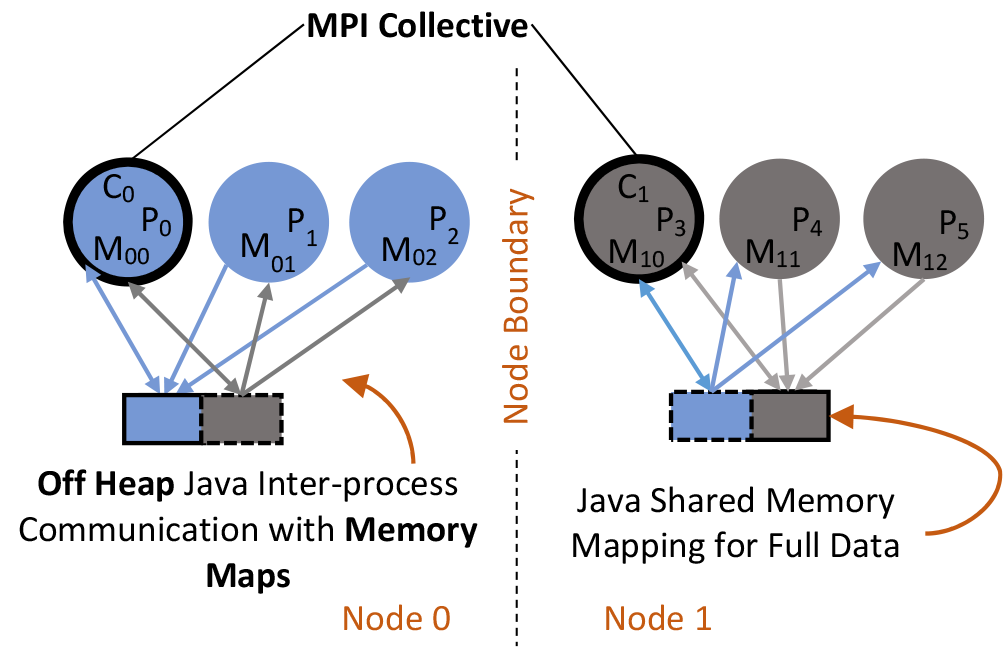
\includegraphics[width=0.9\columnwidth]{figures/fig_mmap_intranode}
\caption{Intra-node message passing with Java shared memory maps}
\label{fig:fig_mmap_intranode}
\end{figure}

\begin{figure}[!h]
\centering
\includegraphics[width=0.9\columnwidth]{figures/fig_mmap_intranode_het}
\caption{Heterogeneous shared memory intra-node messaging}
\label{fig:fig_mmap_intranode_het}
\end{figure}

SPIDAL Java's shared memory intra-node communication uses a custom memory maps implementation from OpenHFT's JavaLang\cite{openhftjavalang} project to perform inter-process communication for processes within a node, thus eliminating any intra-node MPI calls. The standard MPI programming would require $O(R^2)$ of communications in a collective call, where $R$ is the number of processes. In this optimization, we have effectively reduced this to $O(\hat{N}^2)$, where $\hat{N}$ is the number of nodes. Note this is an application level optimization rather than an improvement to a particular MPI implementation, thus, it will be possible for SPIDAL Java to be ported for future MPI Java bindings with minimal changes.  

Figure \ref{fig:fig_mmap_intranode} shows the general architecture of this optimization where two nodes, each with three processes, are used as an example. Process ranks go from $P_0$ to $P_5$ and belong to \texttt{MPI\_COMM\_WORLD}. One process from each node acts as the communication leader - $C_0$ and $C_1$. These leaders have a separate MPI communicator called \texttt{COLLECTIVE\_COMM}. Similarly, processes within a node belong to a separate \texttt{MMAP\_COMM}, for example, $M_{00}$ to $M_{02}$ in one communicator for node 0 and $M_{10}$ to $M_{12}$ in another for node 1. Also, all processes within a node map the same memory region as an off-heap buffer in Java and compute necessary offsets at the beginning of the program. The takeaway point of this setup is the use of memory maps to communicate between processes and the reduction in communication  calls. A typical call to an MPI collective will internally go through the following modified steps.

\begin{enumerate}
\item All processes, $P_0$ to $P_5$, write their partial data to the mapped memory region offset by their rank and node. See downward blue arrows for node 0 and gray arrows for node 1 in the figure.
\item Communication leaders, $C_0$ and $C_1$, wait for the peers, $\{M_{01},M_{02}\}$ and $\{M_{10},M_{11}\}$ to finish writing. Note leaders wait only for their peers in the same node.
\item Once the partial data is written, the leaders participate in the MPI collective call with partial data from their peers - upward blue arrows for node 0 and gray arrows for node 1. Also, the leaders may perform the collective operation locally on the partial data and use its results for the MPI communication depending on the type of collective required. MPI \texttt{allgatherv}, for example, will not have any local operation to be performed, but something like \texttt{allreduce} may benefit from doing the reduction locally. Note, the peers wait while their leader performs MPI communication.
\item At the end of the MPI communication, the leaders write the results to the respective memory maps - downward gray arrows for node 0 and blue arrows for node 1. This data is then immediately available to their peers without requiring further communication - upward gray arrows for node 0 and blue arrows for node 1.
\end{enumerate}

This approach reduces MPI communication to just 2 processes, in contrast to a typical MPI program, where 6 processes would be communicating with each other. The two wait operations mentioned above can be implemented using memory mapped variables or with an MPI \texttt{barrier} on the \texttt{MMAP\_COMM}; although the latter will cause intra-node messaging, experiments showed it to incur negligible costs compared to actual data communication.

% \begin{figure}[!h]
% \centering
% \includegraphics[width=0.9\columnwidth]{fig_mmap_intranode_het}
% \caption{Heterogeneous shared memory intra-node messaging}
% \label{fig:fig_mmap_intranode_het}
% \end{figure}

While the uniform rank distribution across nodes and a single memory map group per node in Figure \ref{fig:fig_mmap_intranode} is the optimal pattern to reduce communication, SPIDAL supports two heterogeneous settings as well. Figure \ref{fig:fig_mmap_intranode_het} shows these two modes.

\textbf{Non-uniform rank distribution} - Juliet HPC cluster, for example, has two groups of nodes with different core counts (24 and 36) per node. SPIDAL Java supports different process counts per node to utilize all available cores in situations like this. Also, it automatically detects the heterogeneous configurations and adjusts its shared memory buffers accordingly.

\textbf{Multiple memory groups per node} - If more than 1 memory map per node ($M$) is specified, SPIDAL Java will select one communication leader per group even for groups within the same node. Figure \ref{fig:fig_mmap_intranode_het} shows 2 memory maps per node. As a result, $O(\hat{N}^2)$ communication is now changed to $O((\hat{N}M)^2)$, so it is highly recommended to use a smaller $M$, ideally, $M=1$.


\subsection{Cache and Memory Utilization}
While this is a generic performance consideration in computing, big data applications iterating over large arrays suffer significant performance loss if not properly utilized. SPIDAL Java employs 3 classic techniques from the linear algebra domain to improve cache and memory costs  - blocked loops, 1D arrays, and loop ordering. 

\textbf{Blocked loops} - Nested loops that access matrix structures use blocking such that the chunks of data will fit in cache and reside there for the duration of its use. 

\textbf{1D arrays for 2D data} - 2D arrays representing 2D data require 2 indirect memory references to get an element. This is significant with increasing data sizes, so SPIDAL Java uses 1D arrays to represent 2D data. As such with 1 memory reference and computed indices, it can access 2D data efficiently. This also improves cache utilization as 1D arrays are contiguous in memory.

\textbf{Loop ordering} - Data decomposition in SPIDAL Java blocks full data into rectangular matrices, so to efficiently use cache, it restructures nested loops that access these to go along the longest dimension within the inner loop. Note, this is necessary only when 2D array representation is necessary. 

\subsection{The Cost of Java Threads}
While many of the big data frameworks employ threads to execute tasks, a comparison of performance against processes is not available for big data applications. SPIDAL Java applications support the hybrid approach of threads within MPI to create parallel \texttt{for} regions using Habanero Java library \cite{Imam:2014:HLJ:2647508.2647514}. Note, threads perform computations only and do not invoke MPI operations. The parent process aggregates the results from threads locally as appropriate before using it in collective communications. Also, the previous shared memory messaging adds a second level of result aggregation within processes of the same node to further reduce communication. Figure~\ref{fig:fig_thread_parallelism} shows the usage of threads in SPIDAL Java with different levels of result aggregation. 

\begin{figure}
\centering
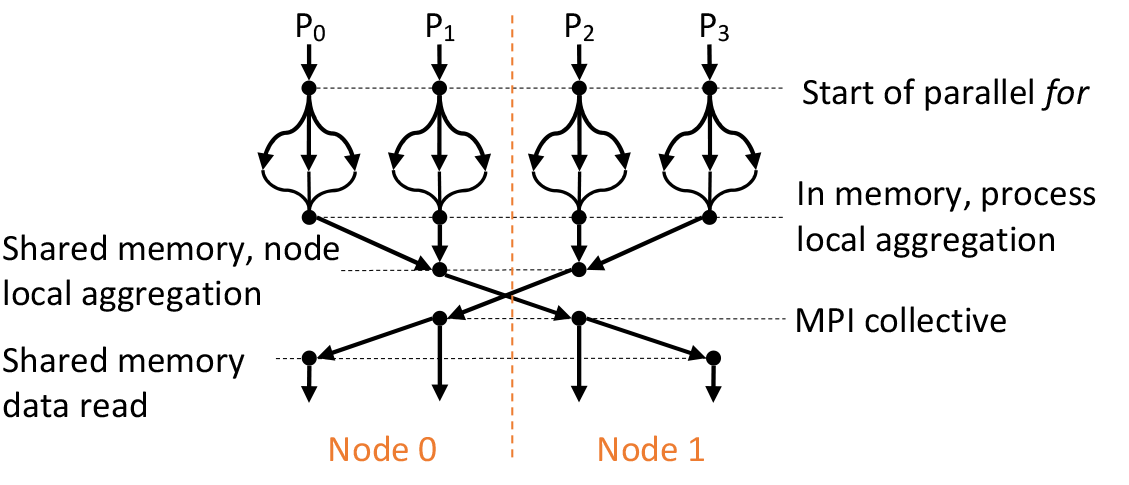
\includegraphics[width=0.9\columnwidth]{figures/fig_thread_parallelism}
\caption{The architecture of utilizing threads for intra-process parallelism}
\label{fig:fig_thread_parallelism}
\end{figure}

Applications decompose data at the process level first and split further for threads. This guarantees that threads operate on non-conflicting data arrays; however, Figure \ref{fig:fig_100K_TP}, \ref{fig:fig_200K_TP}, and \ref{fig:fig_400K_TP} show a rapid degrade in performance with increasing number of threads per process. Internal timings of the code suggest poor performance occurs in computations with arrays, which suggests possible false sharing and suboptimal cache usage. Therefore, while the communication bottleneck with default MPI implementations favored the use of threads, with shared memory intra-node messaging optimization in SPIDAL Java they offer no advantage, hence, processes are a better choice than threads for these applications.

\subsection{The Overhead of Garbage Collection}
It is critical to maintain a minimal memory footprint and reduce memory management costs in performance sensitive applications with large memory requirements such as those in SPIDAL Java. The Java Virtual Machine (JVM) automatically manages memory allocations and performs GC to reduce memory growth. It does so by segmenting the program's heap into regions called generations, and moving objects between these regions depending on their longevity. Every object starts in Young Generation (YG) and gets promoted to Old Generation (OG) if they have lived long enough. Minor garbage collections happen in YG frequently and short-lived objects are removed without GC going through the entire Heap. Also, long-lived objects are moved to the OG. When OG has reached its maximum capacity, a full GC happens, which is an expensive operation depending on the size of the heap and can take considerable time. Also, both minor and major collections have to stop all the threads running in the process while moving the objects. Such GC pauses incur significant delays, especially for GML applications where slowness in one process affects all others as they have to synchronize on global communications. 

Initial versions of SPIDAL Java followed the standard Object Oriented Programming (OOP), where objects were created as and when necessary while letting GC take care of the heap. The performance results, however, showed inconsistent behavior, and detailed GC log analysis revealed processes were paused most of the time to perform GC. Also, the max heap required (JVM -Xmx setting) to get reasonable timing quickly surpassed the physical memory in Juliet cluster with increasing data sizes.

The optimization to overcome these memory challenges was to compute the total memory allocation required for a given data size and statically allocate required arrays. Also, the computation codes reuse these arrays creating no garbage. Another optimization is to use off-heap buffers for communications and other static data, which is discussed in the next subsection.

While precomputing memory requirements is application dependent, static allocation and array reuse can bring down GC costs to negligible levels. Benefits of this approach in SPIDAL Java are as follows.

\textbf{Zero GC} - Objects are placed in the OG and no transfer of objects from YG to OG happens in run-time, which avoids full GC.

\textbf{Predictable performance} - With GC out of the way, the performance numbers agreed with expected behavior of increasing data and parallelism.

\textbf{Reduction in memory footprint} - A DA-MDS run of 200K points running with 1152 way parallelism required about 5GB heap per process or 120 GB per node (24 processes on 1 node), which hits the maximum memory per node in our cluster, which is 128GB. The improved version required less than 1GB per process for the same parallelism, giving about 5x improvement on memory footprint. 

\subsection{The Cost of Heap Allocated Objects}
With traditional heap allocated objects, the JVM has to make extra copies whenever a native operation is performed on it. One reason for this is  JVM cannot guarantee that the memory reference to a buffer will stay intact during a native call because it is possible for a GC compaction to happen and move the buffer to a different place in the heap. The solution employed in SPIDAL Java is to use direct buffers, which are off-heap data structures, that allows the JVM to perform fast native operations without data copying. 

SPIDAL Java uses off-heap buffers efficiently for the following 3 tasks.

\textbf{Initial data loading} - Input data in SPIDAL Java are $NxN$ binary matrices stored in 16-byte (short) big-endian or little-endian format. Java stream APIs such as the typical $DataInputStream$ class are very inefficient in loading these matrices. Instead, SPIDAL Java memory maps these matrices (each process maps only the chunk it operates on) as Java direct buffers.

\textbf{Intra-node messaging} - Intra-node process-to-process communications happen through custom off heap memory maps, thus avoiding MPI within a node. While Java memory maps allow multiple processes to map the same memory region, it does not guarantee writes from one process will be visible to the other immediately. The OpenHFT Java Lang Bytes \cite{openhftjavalang} used here is an efficient off-heap buffer implementation, which guarantees write consistency. 

\textbf{MPI communications} - While OpenMPI supports both on- and off-heap buffers for communication, SPIDAL Java uses statically allocated direct buffers, which greatly reduce the cost of MPI communication calls. 